\documentclass{article}
\usepackage[paperwidth=360pt,paperheight=245pt,margin=0pt,noheadfoot]{geometry}
\usepackage{tikz}
\usetikzlibrary{calc}

\definecolor{ink}{RGB}{28,41,56}
\definecolor{axis}{RGB}{100,116,139}
\definecolor{grid}{RGB}{203,213,225}
\definecolor{curve}{RGB}{30,64,175}
\definecolor{teal}{RGB}{13,148,136}
\definecolor{tealfill}{RGB}{176,227,219}
% Integral diagrams have one consistent three-colour vocabulary: blue for an
% under-only part, yellow for an over-only (or still-unresolved) part, and
% green for their common part.  The common part is explicit rather than an
% alpha blend, so it remains visibly distinct after GIF palette quantization.
\definecolor{cyan}{RGB}{0,84,134}
\definecolor{cyanfill}{RGB}{0,114,178}
\definecolor{yellow}{RGB}{184,134,11}
\definecolor{yellowfill}{RGB}{240,228,66}
\definecolor{overlap}{RGB}{15,110,67}
\definecolor{overlapfill}{RGB}{20,153,92}
\definecolor{orange}{RGB}{234,88,12}
\definecolor{orangefill}{RGB}{254,215,170}
\definecolor{purple}{RGB}{126,34,206}
\definecolor{yellowedge}{RGB}{202,138,4}
\definecolor{projection}{RGB}{148,163,184}
\colorlet{under}{cyan}
\colorlet{underfill}{cyanfill}
\colorlet{over}{yellow}
\colorlet{overfill}{yellowfill}
\colorlet{shared}{overlap}
\colorlet{sharedfill}{overlapfill}
\colorlet{gap}{yellow}
\colorlet{gapfill}{yellowfill}

\pagestyle{empty}
\setlength\parindent{0pt}
\setlength\topskip{0pt}
\begin{document}
\noindent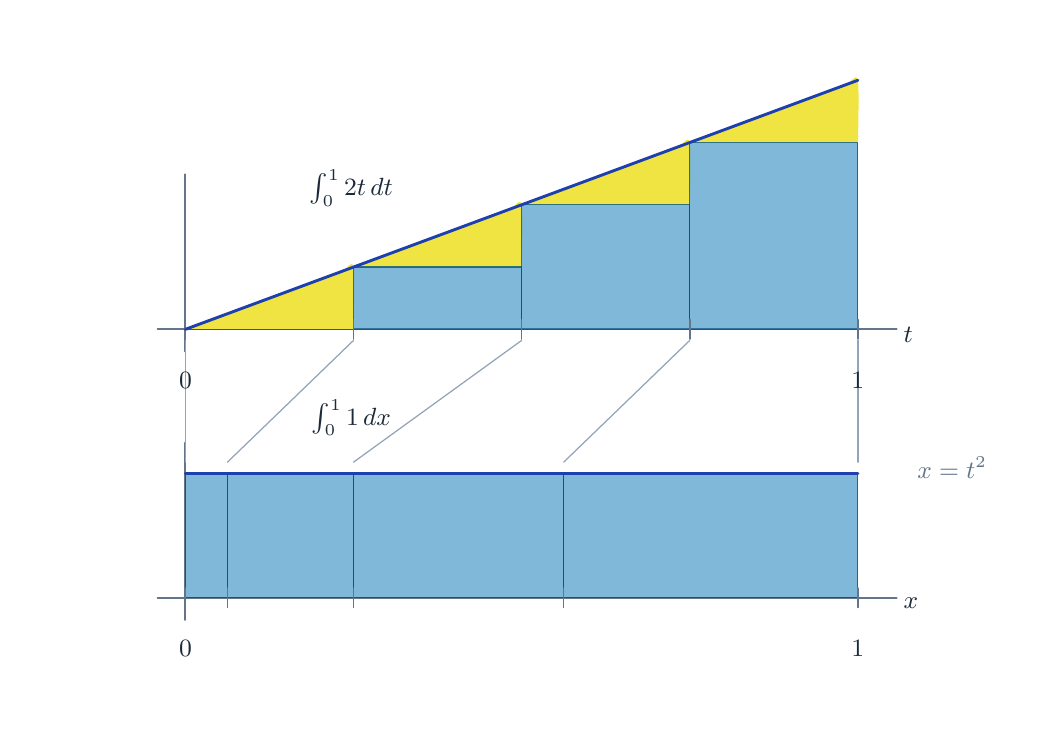
\begin{tikzpicture}[baseline=(current bounding box.north),x=1pt,y=1pt,line cap=round,line join=round]
\useasboundingbox (0,0) rectangle (360,245);
\draw[axis,line width=.75pt] (47,136) -- (314,136);
\draw[axis,line width=.75pt] (57,128) -- (57,192);
\draw[axis,line width=.75pt] (47,39) -- (314,39);
\draw[axis,line width=.75pt] (57,31) -- (57,95);
\path[fill=gapfill] plot[smooth] coordinates {(57,136) (57,136) (60.7969,137.4062) (64.5938,138.8125) (68.3906,140.2188) (72.1875,141.625) (75.9844,143.0312) (79.7812,144.4375) (83.5781,145.8438) (87.375,147.25) (91.1719,148.6562) (94.9688,150.0625) (98.7656,151.4688) (102.5625,152.875) (106.3594,154.2812) (110.1562,155.6875) (113.9531,157.0938) (117.75,158.5) (117.75,136)} -- cycle;
\path[fill=underfill,fill opacity=.5,draw=under,draw opacity=.8,line width=.4pt] (57,136) rectangle (117.75,136);
\path[fill=underfill,fill opacity=.5,draw=under,draw opacity=.8,line width=.4pt] (57,39) rectangle (72.1875,84);
\path[fill=gapfill] plot[smooth] coordinates {(117.75,158.5) (117.75,158.5) (121.5469,159.9062) (125.3438,161.3125) (129.1406,162.7188) (132.9375,164.125) (136.7344,165.5312) (140.5312,166.9375) (144.3281,168.3438) (148.125,169.75) (151.9219,171.1562) (155.7188,172.5625) (159.5156,173.9688) (163.3125,175.375) (167.1094,176.7812) (170.9062,178.1875) (174.7031,179.5938) (178.5,181) (178.5,158.5)} -- cycle;
\path[fill=underfill,fill opacity=.5,draw=under,draw opacity=.8,line width=.4pt] (117.75,136) rectangle (178.5,158.5);
\path[fill=underfill,fill opacity=.5,draw=under,draw opacity=.8,line width=.4pt] (72.1875,39) rectangle (117.75,84);
\path[fill=gapfill] plot[smooth] coordinates {(178.5,181) (178.5,181) (182.2969,182.4062) (186.0938,183.8125) (189.8906,185.2188) (193.6875,186.625) (197.4844,188.0312) (201.2812,189.4375) (205.0781,190.8438) (208.875,192.25) (212.6719,193.6562) (216.4688,195.0625) (220.2656,196.4688) (224.0625,197.875) (227.8594,199.2812) (231.6562,200.6875) (235.4531,202.0938) (239.25,203.5) (239.25,181)} -- cycle;
\path[fill=underfill,fill opacity=.5,draw=under,draw opacity=.8,line width=.4pt] (178.5,136) rectangle (239.25,181);
\path[fill=underfill,fill opacity=.5,draw=under,draw opacity=.8,line width=.4pt] (117.75,39) rectangle (193.6875,84);
\path[fill=gapfill] plot[smooth] coordinates {(239.25,203.5) (239.25,203.5) (243.0469,204.9062) (246.8438,206.3125) (250.6406,207.7188) (254.4375,209.125) (258.2344,210.5312) (262.0312,211.9375) (265.8281,213.3438) (269.625,214.75) (273.4219,216.1562) (277.2188,217.5625) (281.0156,218.9688) (284.8125,220.375) (288.6094,221.7812) (292.4062,223.1875) (296.2031,224.5938) (300,226) (300,203.5)} -- cycle;
\path[fill=underfill,fill opacity=.5,draw=under,draw opacity=.8,line width=.4pt] (239.25,136) rectangle (300,203.5);
\path[fill=underfill,fill opacity=.5,draw=under,draw opacity=.8,line width=.4pt] (193.6875,39) rectangle (300,84);
\draw[projection,line width=.45pt] (57,132) -- (57,88);
\draw[axis,line width=.55pt] (57,132.5) -- (57,139.5);
\draw[axis,line width=.55pt] (57,35.5) -- (57,42.5);
\draw[projection,line width=.45pt] (117.75,132) -- (72.1875,88);
\draw[axis,line width=.55pt] (117.75,132.5) -- (117.75,139.5);
\draw[axis,line width=.55pt] (72.1875,35.5) -- (72.1875,42.5);
\draw[projection,line width=.45pt] (178.5,132) -- (117.75,88);
\draw[axis,line width=.55pt] (178.5,132.5) -- (178.5,139.5);
\draw[axis,line width=.55pt] (117.75,35.5) -- (117.75,42.5);
\draw[projection,line width=.45pt] (239.25,132) -- (193.6875,88);
\draw[axis,line width=.55pt] (239.25,132.5) -- (239.25,139.5);
\draw[axis,line width=.55pt] (193.6875,35.5) -- (193.6875,42.5);
\draw[projection,line width=.45pt] (300,132) -- (300,88);
\draw[axis,line width=.55pt] (300,132.5) -- (300,139.5);
\draw[axis,line width=.55pt] (300,35.5) -- (300,42.5);
\draw[curve,line width=1.05pt] plot[smooth] coordinates {(57,136) (60.0375,137.125) (63.075,138.25) (66.1125,139.375) (69.15,140.5) (72.1875,141.625) (75.225,142.75) (78.2625,143.875) (81.3,145) (84.3375,146.125) (87.375,147.25) (90.4125,148.375) (93.45,149.5) (96.4875,150.625) (99.525,151.75) (102.5625,152.875) (105.6,154) (108.6375,155.125) (111.675,156.25) (114.7125,157.375) (117.75,158.5) (120.7875,159.625) (123.825,160.75) (126.8625,161.875) (129.9,163) (132.9375,164.125) (135.975,165.25) (139.0125,166.375) (142.05,167.5) (145.0875,168.625) (148.125,169.75) (151.1625,170.875) (154.2,172) (157.2375,173.125) (160.275,174.25) (163.3125,175.375) (166.35,176.5) (169.3875,177.625) (172.425,178.75) (175.4625,179.875) (178.5,181) (181.5375,182.125) (184.575,183.25) (187.6125,184.375) (190.65,185.5) (193.6875,186.625) (196.725,187.75) (199.7625,188.875) (202.8,190) (205.8375,191.125) (208.875,192.25) (211.9125,193.375) (214.95,194.5) (217.9875,195.625) (221.025,196.75) (224.0625,197.875) (227.1,199) (230.1375,200.125) (233.175,201.25) (236.2125,202.375) (239.25,203.5) (242.2875,204.625) (245.325,205.75) (248.3625,206.875) (251.4,208) (254.4375,209.125) (257.475,210.25) (260.5125,211.375) (263.55,212.5) (266.5875,213.625) (269.625,214.75) (272.6625,215.875) (275.7,217) (278.7375,218.125) (281.775,219.25) (284.8125,220.375) (287.85,221.5) (290.8875,222.625) (293.925,223.75) (296.9625,224.875) (300,226)};
\draw[curve,line width=1.05pt] (57,84) -- (300,84);
\node[font=\small,text=ink,anchor=north] at (57,124) {$0$};
\node[font=\small,text=ink,anchor=north] at (300,124) {$1$};
\node[font=\small,text=ink,anchor=north] at (57,27) {$0$};
\node[font=\small,text=ink,anchor=north] at (300,27) {$1$};
\node[font=\small,text=ink,anchor=west] at (313,134) {$t$};
\node[font=\small,text=ink,anchor=west] at (313,37) {$x$};
\node[font=\small,text=ink,anchor=south] at (117,177) {$\int_0^1 2t\,dt$};
\node[font=\small,text=ink,anchor=south] at (117,94) {$\int_0^1 1\,dx$};
\node[font=\small,text=ink,anchor=west,text=axis] at (318,86) {$x=t^2$};
\end{tikzpicture}
\end{document}
